\documentclass[11pt,a4paper]{article}
\usepackage[T1]{fontenc}
\usepackage[utf8]{inputenc}
\usepackage{lmodern}
\usepackage[margin=1in]{geometry}
\usepackage{amsmath}
\usepackage{amssymb}
\usepackage{graphicx}
\usepackage{array}
\usepackage{booktabs}
\usepackage{longtable}
\usepackage{hyperref}

\title{PX4 Python SITL: Dynamics, Vehicle Models, Sensors, Forces, and External Interfaces}
\author{PX4 Python SITL}
\date{\today}

\begin{document}
\maketitle
\tableofcontents
\clearpage

\section{Scope}
This document describes the simulation kernel and interfaces implemented in the repository:
\begin{itemize}
    \item 6DOF rigid-body kernel and integration flow,
    \item vehicle model parameterizations (\texttt{x8}, \texttt{iris}, \texttt{ts06}),
    \item force and moment models per vehicle,
    \item sensor models (IMU, magnetometer, barometer, GPS),
    \item communication with PX4 over MAVLink and with external programs over UDP/WebSocket.
\end{itemize}
Frames used are NED for navigation and FRD for body axes.

\section{Variable Inventory}
Table \ref{tab:variables} lists symbols used in equations, including units and dimensions.

\footnotesize
\renewcommand{\arraystretch}{1.12}
\begin{longtable}{>{\raggedright\arraybackslash}p{0.16\textwidth} >{\raggedright\arraybackslash}p{0.34\textwidth} >{\raggedright\arraybackslash}p{0.18\textwidth} >{\raggedright\arraybackslash}p{0.12\textwidth} >{\raggedright\arraybackslash}p{0.12\textwidth}}
\caption{Variables, default values, units, and dimensions}\label{tab:variables}\\
\toprule
Symbol & Meaning & Default & Unit & Dimension \\
\midrule
\endfirsthead
\toprule
Symbol & Meaning & Default & Unit & Dimension \\
\midrule
\endhead
$y$ & full simulation state vector & set by initial condition and integration & mixed & mixed \\
$\dot{y}$ & state derivative vector & computed each step & mixed & mixed \\
$p_{ned}=[p_n,p_e,p_d]^T$ & position in local North-East-Down frame & initial $[0,0,-3]$ in main loop & m & $L$ \\
$v_b=[u,v,w]^T$ & body-frame linear velocity (FRD) & initial $[0,0,0]$ & m/s & $LT^{-1}$ \\
$v_{ned}$ & NED velocity & derived from $R_{bw}v_b$ & m/s & $LT^{-1}$ \\
$\omega_b=[p,q,r]^T$ & body-frame angular velocity & initial $[0,0,0]$ & rad/s & $T^{-1}$ \\
$q=[q_w,q_x,q_y,q_z]^T$ & attitude quaternion used in kernel & default identity $[1,0,0,0]$ & 1 & 1 \\
$R_{wb}(q)$ & world-to-body rotation matrix & derived from $q$ & 1 & 1 \\
$R_{bw}$ & body-to-world rotation matrix ($R_{wb}^T$) & derived from $q$ & 1 & 1 \\
$f_b=[F_x,F_y,F_z]^T$ & net body force & sum of active and passive models & N & $MLT^{-2}$ \\
$m_b=[M_x,M_y,M_z]^T$ & net body moment & sum of active and passive models & N m & $ML^2T^{-2}$ \\
$I$ & inertia matrix at center of gravity & vehicle specific (Iris: diag$(5e$-$3,5e$-$3,9e$-$3)$) & kg m$^2$ & $ML^2$ \\
$m$ & vehicle mass & vehicle specific (Iris: $1.5$) & kg & $M$ \\
$g$ & gravity magnitude & $9.81$ & m/s$^2$ & $LT^{-2}$ \\
$g_w$ & gravity vector in world frame for IMU model & $[0,0,-9.8068]$ & m/s$^2$ & $LT^{-2}$ \\
$a_b$ & body translational acceleration & computed each step & m/s$^2$ & $LT^{-2}$ \\
$a_{imu,in}$ & acceleration fed to IMU model & $\dot{v}_b+\omega_b\times v_b$ & m/s$^2$ & $LT^{-2}$ \\
$f_{spec}$ & specific force before IMU filtering/noise & computed each step & m/s$^2$ & $LT^{-2}$ \\
$\tau_a,\tau_g$ & IMU filter time constants & from $f_c=120$ Hz ($\tau\approx1.326$ ms) & s & $T$ \\
$f_{c,acc}, f_{c,gyro}$ & IMU LPF cutoff frequencies & $120,120$ & Hz & $T^{-1}$ \\
$f_{imu}, f_{mag}, f_{baro}, f_{gps}$ & sensor update rates (IMU/Mag/Baro/GPS) & $250,100,20,5$ & Hz & $T^{-1}$ \\
$\alpha_a,\alpha_g$ & LPF update coefficients & computed from $\Delta t$ and $\tau$ & 1 & 1 \\
$b_a,b_g,b_m$ & accel/gyro/mag bias states & initialized from sensor bias settings & sensor unit & sensor dimension \\
$n_a,n_g,n_m,n_P,n_q$ & additive white-noise terms & zero mean (noise enabled) & sensor unit & sensor dimension \\
$\sigma_{acc},\sigma_{gyro}$ & IMU continuous noise densities & from IMU defaults & m/s$^2$/\(\sqrt{\text{Hz}}\), rad/s/\(\sqrt{\text{Hz}}\) & sensor dimension $T^{-1/2}$ \\
$\sigma_{a,d},\sigma_{\omega,d}$ & IMU discrete noise std. dev. & $\sigma/\sqrt{\Delta t}$ & m/s$^2$, rad/s & sensor dimension \\
$\sigma_{ba,d},\sigma_{bg,d},\sigma_{bm,d}$ & discrete bias-innovation std. dev. (acc/gyro/mag) & computed from $rw$ and $\tau_c$ & sensor unit & sensor dimension \\
$rw_{acc}, rw_{gyro}, rw_{mag}$ & bias random-walk amplitudes & defaults in IMU/Mag classes & sensor unit\(\sqrt{\text{Hz}}\) & sensor dimension $T^{-1/2}$ \\
$\sigma_{mag},\sigma_P$ & magnetometer/barometer noise level & defaults in sensor classes & gauss/\(\sqrt{\text{Hz}}\), Pa & sensor dimension \\
$\sigma_{xy},\sigma_z,\sigma_{vxy},\sigma_{vz}$ & GPS pos/vel noise densities & defaults in GPS class & m/\(\sqrt{\text{Hz}}\), m/s/\(\sqrt{\text{Hz}}\) & sensor dimension $T^{-1/2}$ \\
$\phi_a,\phi_g,\phi_m$ & Gauss-Markov persistence terms & $\exp(-\Delta t/\tau_c)$ & 1 & 1 \\
$\eta_{ba},\eta_{bg},\eta_{bm}$ & Gauss-Markov innovation terms & zero mean Gaussian draws & sensor unit & sensor dimension \\
$w_i$ & GPS bias-driving random-walk term ($i\in\{N,E,D\}$) & sampled Gaussian process & m/s & $LT^{-1}$ \\
$m_{ned}=[m_N,m_E,m_D]^T$ & Earth magnetic field vector in NED & model default $[0.215,0.010,0.430]$ & gauss & magnetic flux density \\
$H,X,Y,Z$ & intermediate magnetic components used to form $m_{ned}$ & computed from $\delta,\iota,B_0$ & gauss & magnetic flux density \\
$\delta,\iota,B_0$ & magnetic declination, inclination, field strength & $0.0391,1.1345,0.475$ & rad,rad,gauss & 1,1,magnetic flux density \\
$S_{si}$ & soft-iron calibration matrix & identity $I_3$ & 1 & 1 \\
$b_{hi}$ & hard-iron offset vector & from model mag bias (default zero) & gauss & magnetic flux density \\
$z_{local}$ & barometer altitude input & $-p_d$ & m & $L$ \\
$h_0$ & home altitude (AMSL) & GPS model set-home altitude (default $488$, often overridden by model origin) & m & $L$ \\
$h_{amsl}$ & current altitude above mean sea level & $h_0+z_{local}$ & m & $L$ \\
$T_0,T$ & ISA reference/current temperature & $T_0=288.15$, $T$ computed & K & $\Theta$ \\
$P_0,P_{ideal},P_{meas}$ & pressure terms in barometer model & $P_0=101325$, others computed & Pa & $ML^{-1}T^{-2}$ \\
$\rho_{air},\rho_{baro}$ & air density terms & $\rho_{air}=1.225$, $\rho_{baro}$ computed & kg/m$^3$ & $ML^{-3}$ \\
$L$ & ISA temperature lapse rate & $0.0065$ & K/m & $\Theta L^{-1}$ \\
$d_P$ & accumulated barometer pressure drift & initialized $0$ & Pa & $ML^{-1}T^{-2}$ \\
$r_{drift}$ & barometer pressure drift rate & SensorSuite default $0.05$ & Pa/s & $ML^{-1}T^{-3}$ \\
$R_E$ & Earth radius in GPS reprojection & $6{,}371{,}000$ & m & $L$ \\
$\varphi,\lambda$ & latitude and longitude & computed by reprojection & rad & 1 \\
$\varphi_0,\lambda_0$ & GPS origin latitude/longitude & $47.397742^\circ$, $8.545594^\circ$ & rad & 1 \\
$\beta_N,\beta_E,\beta_D$ & GPS position random-walk states & initialized $0$ & m & $L$ \\
$\tau_{gps}$ & GPS bias/random-walk correlation time & $60$ & s & $T$ \\
$\nu_\cdot,\xi_\cdot$ & GPS position and velocity noise terms & zero mean, configured by noise densities & m or m/s & $L$ or $LT^{-1}$ \\
\bottomrule
\end{longtable}
\normalsize

\section{Simulation Kernel}
\subsection{Short Introduction}
The rigid-body kernel in \texttt{src/dynamics/dynamics.py} evolves the 13-state vector under the summed body-frame force and moment input and gravity.
Figure \ref{fig:ned_frd} introduces the coordinate conventions used by the equations: world frame NED (North-East-Down) and body frame FRD (Forward-Right-Down).

\begin{figure}[ht]
    \centering
    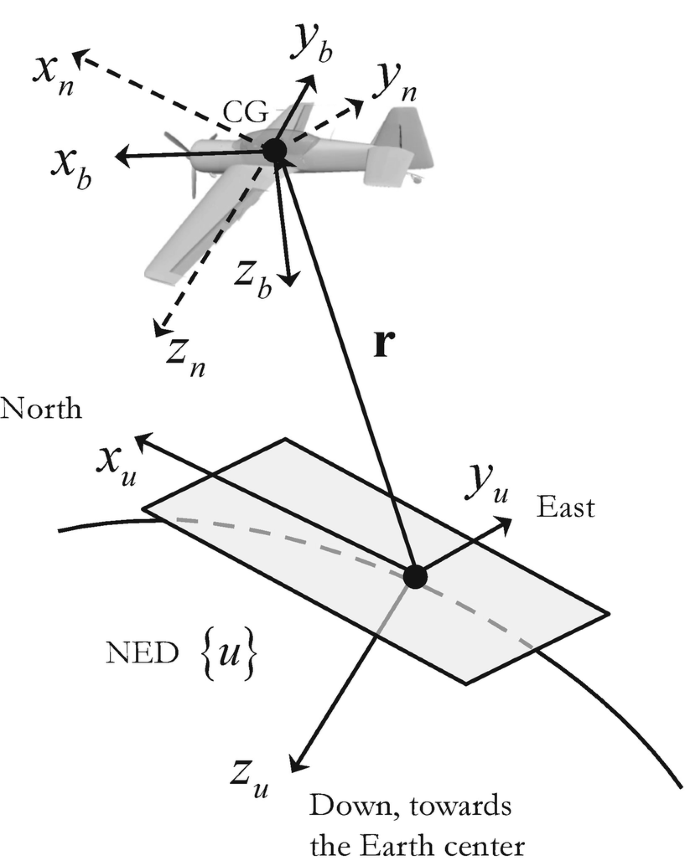
\includegraphics[width=0.72\textwidth]{../media/pic1.png}
    \caption{Coordinate systems used in the simulator: local NED world frame and FRD body frame.}
    \label{fig:ned_frd}
\end{figure}

\subsection{6DOF Model}
\subsubsection{Assumptions}
\begin{itemize}
    \item Constant mass and inertia over one simulation step.
    \item Forces and moments are fully summed in body frame before the dynamics call.
    \item Ground-contact clamp at $z_{ned}=0$: if $p_d\ge0$, then $p_d\leftarrow0$, and downward components are clamped by $v_{ned,D}\leftarrow\min(v_{ned,D},0)$ and $a_{ned,D}\leftarrow\min(a_{ned,D},0)$ before reprojection to body-frame derivatives.
    \item Explicit fixed-step lockstep integration.
\end{itemize}

\subsubsection{Equations}
State and kinematics:
\begin{align}
y &= [p_n,p_e,p_d,q_w,q_x,q_y,q_z,u,v,w,p,q,r]^T, \\
v_b &= [u,v,w]^T, \quad \omega_b=[p,q,r]^T, \\
\dot{p}_{ned} &= R_{bw}(q)\,v_b.
\end{align}

Translational and rotational dynamics:
\begin{align}
f_b &= [F_x,F_y,F_z]^T, \quad m_b=[M_x,M_y,M_z]^T, \\
a_b &= \frac{f_b + R_{wb}(q)[0,0,mg]^T}{m} - \omega_b \times v_b, \\
\dot{\omega}_b &= I^{-1}\left(m_b - \omega_b \times I\omega_b\right).
\end{align}

Attitude dynamics:
\begin{align}
\dot{q} &= \frac{1}{2}\Omega(\omega_b)q,
\end{align}
where, for $\omega_b=[p,q,r]^T$ and $q=[q_w,q_x,q_y,q_z]^T$,
\begin{equation}
\Omega(\omega_b)=
\begin{bmatrix}
0 & -p & -q & -r \\
p & 0 & r & -q \\
q & -r & 0 & p \\
r & q & -p & 0
\end{bmatrix}.
\end{equation}

Numerical integration (applied to all state components):
\begin{equation}
y_{k+1} = y_k + \dot{y}_k\,\Delta t.
\end{equation}
Quaternion normalization is applied after each integration step.

Ground-contact condition at $z_{ned}=0$:
\begin{align}
\text{if } p_d &\ge 0: \\
p_d &\leftarrow 0, \\
v_{ned,D} &\leftarrow \min(v_{ned,D},0), \\
a_{ned,D} &\leftarrow \min(a_{ned,D},0).
\end{align}
The clamped NED velocity and acceleration are reprojected to body-frame derivatives used by the integrator.

\subsubsection{Catapult-Constrained Start Mode}
When catapult start is enabled, \texttt{World} temporarily replaces free 6DOF with a rail-constrained kernel from \texttt{src/dynamics/dynamics.py} (function \texttt{rail\_dynamics}), while catapult pull force is computed in \texttt{src/vehicles/common\_forces/catapult\_rail.py}. Let $\hat r_{rail}^{ned}$ be the unit rail direction and $p_{rail,0}^{ned}$ the rail start point.

Rail progress and switch condition:
\begin{align}
s &= (p^{ned} - p_{rail,0}^{ned})^T \hat r_{rail}^{ned}, \\
\text{if } s &\ge L_{rail} \Rightarrow \text{switch to free 6DOF.}
\end{align}

Launch is additionally gated by an arm-triggered countdown in the runtime loops (CLI and ROS2):
\begin{align}
t_{release} &= t_{arm} + T_{countdown}, \\
\text{dynamics frozen while } t &< t_{release}.
\end{align}
The countdown duration is configured by environment variable
\texttt{SIM\_CATAPULT\_LAUNCH\_COUNTDOWN\_S} (default $3.0$ s).

During constrained mode, translational motion is projected onto the rail:
\begin{align}
\dot p^{ned} &= (v^{ned}\cdot \hat r_{rail}^{ned})\,\hat r_{rail}^{ned}, \\
f_{rail} &= \max\left(0,\,m\,g\,k_{pull}(L_{rail}-s)\right), \\
f_b^{rail} &= R_{wb}(q)\left(f_{rail}\,\hat r_{rail}^{ned}\right), \\
a_b &= \left(\frac{f_b + f_b^{rail} + R_{wb}(q)[0,0,mg]^T}{m}\cdot \hat r_{rail}^{b}\right)\hat r_{rail}^{b}, \\
\dot q &= 0, \qquad \dot\omega_b = 0.
\end{align}
Here $k_{pull}=\texttt{rail\_pull\_max}$ and $\hat r_{rail}^{b}=R_{wb}(q)\hat r_{rail}^{ned}$. Attitude is held aligned to the rail until switch.
So far, the catapult pull model is assumed linear with rail distance ($\propto (L_{rail}-s)$) and clamped to non-negative force.

\subsection{Program Architecture}
The 6DOF model above defines the rigid-body state propagation used by the simulator core. Vehicle-specific force and moment generation is documented in the \textit{Vehicle Models} chapter, where each vehicle contributes its own force-model set through the catalog.

Sensor synthesis is handled by \texttt{SensorSuite} and documented in the \textit{Sensor Models} chapter, including IMU, magnetometer, barometer, GPS, and differential-pressure/airspeed-related channels.

Communication of simulated sensor and state outputs to PX4 (and integration hooks for external tools) is documented in the \textit{MAVLink and External Communication} chapter.

\begin{verbatim}
                          +------------------------------+
                          |            PX4 SITL          |
                          |   EKF + Controllers + Mixer  |
                          +---------------+--------------+
                                          |
                                HIL_ACTUATOR_CONTROLS
                                          |
                                          v
+-------------------------------------------------------------------------+
|                    px4-python-sitl (src/main.py)                        |
| lockstep scheduler | single-instance runtime | MAVLink endpoint      |
+--------------------+-------------------------+-----------------------+
                     |
                     | controls_to_u()
                     v
            +-------------------+
            | vehicle.World     |
            | state y, ydot,tau |
            +---------+---------+
                      |
        +-------------+--------------+
        |                            |
        v                            v
+---------------+          +----------------------+
| Force Models  |          | Dynamics6DOF Kernel  |
| (by vehicle)  |          | y, ydot = f(y,tau,P) |
+-------+-------+          +----------+-----------+
        |                             |
        +------------- tau -----------+
                                      |
                     +----------------+------------------+
                     |                                   |
                     v                                   v
          +----------------------+            +------------------+
          | GroundTruth WS JSON  |<-----------| SensorSuite      |
          | websockerPublisher   |            | IMU MAG BARO GPS |
          +----------+-----------+            +--------+---------+
                     ^                                   |
                     |                                   v
                     |                    +--------------------------------------+
                     +--------------------| HIL_SENSOR / HIL_GPS / HIL_STATE... |
                                          +--------------------------------------+
                                                          |
                                                          v
                                                        PX4 SITL

                     (ground-truth outputs from Dynamics6DOF/SensorSuite)
\end{verbatim}

\section{Sensor Models}
Sensor synthesis is implemented in \texttt{src/sensors/sensors.py}. Noise is enabled by default for IMU, magnetometer, GPS, and barometer.

\subsection{IMU (Accelerometer + Gyroscope)}
The IMU model in \texttt{src/sensors/imu.py} converts state and state derivative into specific-force and angular-rate measurements with LPF, bias dynamics, and additive noise.

\subsubsection*{Readable Derivation}
\paragraph{1) Frames and core inertial quantities}
\begin{align}
a_{imu,in} &= [\dot{u},\dot{v},\dot{w}]^T + \omega_b \times v_b, \\
g_b &= R_{wb}(q)[0,0,-g]^T, \\
f_{spec} &= a_{imu,in} + g_b.
\end{align}
The $+\,\omega_b\times v_b$ term is required because $[\dot{u},\dot{v},\dot{w}]^T$ is a derivative in a rotating body frame. Using the transport theorem,
\begin{equation}
\left(\frac{d v_b}{dt}\right)_{inertial}=\left(\frac{d v_b}{dt}\right)_{body}+\omega_b\times v_b,
\end{equation}
and from 6DOF translational dynamics
\begin{equation}
a_b=\frac{f_b + R_{wb}(q)[0,0,mg]^T}{m}-\omega_b\times v_b,
\end{equation}
we get
\begin{equation}
a_b+\omega_b\times v_b=\frac{f_b + R_{wb}(q)[0,0,mg]^T}{m},
\end{equation}
which is exactly the force-per-mass term required by the IMU specific-force model. Here specific force means non-gravitational acceleration measured by the accelerometer, i.e. acceleration due to contact/propulsive/aerodynamic forces per unit mass.

\paragraph{Characteristic values (current parameterization)}
The table symbols are tied to the IMU equations through
\begin{align}
f_{imu} &= \frac{1}{\Delta t}, \\
\tau_a &= \frac{1}{2\pi f_{c,acc}}, \quad \tau_g = \frac{1}{2\pi f_{c,gyro}}, \\
\sigma_{a,d} &= \frac{\sigma_{acc}}{\sqrt{\Delta t}}, \quad \sigma_{\omega,d} = \frac{\sigma_{gyro}}{\sqrt{\Delta t}}.
\end{align}
\begin{center}
\begin{tabular}{llll}
\toprule
Variable & Description & Value & Unit \\
\midrule
$f_{imu}$ & update rate & $250$ & Hz \\
$f_{c,acc}$ & accelerometer LPF cutoff & $120$ & Hz \\
$f_{c,gyro}$ & gyroscope LPF cutoff & $120$ & Hz \\
$\sigma_{acc}$ & accelerometer noise density & $4.0\times10^{-3}$ & m/s$^2$/\(\sqrt{\text{Hz}}\) \\
$\sigma_{gyro}$ & gyroscope noise density & $3.3937\times10^{-4}$ & rad/s/\(\sqrt{\text{Hz}}\) \\
$rw_{acc}$ & accelerometer bias random walk & $6.0\times10^{-3}$ & m/s$^2\sqrt{\text{Hz}}$ \\
$rw_{gyro}$ & gyroscope bias random walk & $3.8785\times10^{-5}$ & rad/s\(\sqrt{\text{Hz}}\) \\
$\tau_{ca}$ & accelerometer bias correlation time & $300$ & s \\
$\tau_{cg}$ & gyroscope bias correlation time & $1000$ & s \\
$a_{max}$ & accelerometer range & $\pm18g$ & m/s$^2$ \\
$\omega_{max}$ & gyroscope range & $\pm2000$ & deg/s \\
\bottomrule
\end{tabular}
\end{center}

\paragraph{Flow chart}
{\footnotesize
\begin{verbatim}
[Input] y, ydot, q
    |
    v
[Core]  a_imu_in -> f_spec
        ([u_dot,v_dot,w_dot] + omega x v) + g_b
    |
    v
[Model] LPF -> bias/noise -> saturation
    |
    v
[Output] HIL_SENSOR.accel + HIL_SENSOR.gyro

Trigger: SensorSuite.update() on each world update tick.
Rate:    nominal f_imu = 250 Hz (model dt fallback).
Gate:    none (no next_update_us gate in IMU class).
\end{verbatim}
}

\paragraph{2) Sensor shaping (LPF + bias + noise)}
\begin{align}
f_{lpf}(k) &= f_{lpf}(k-1)+\alpha_a\left(f_{spec}(k)-f_{lpf}(k-1)\right), \\
\omega_{lpf}(k) &= \omega_{lpf}(k-1)+\alpha_g\left(\omega_b(k)-\omega_{lpf}(k-1)\right), \\
\alpha_{a,g} &= \frac{\Delta t}{\tau_{a,g}+\Delta t}, \\
b_a(k) &= \phi_a b_a(k-1)+\eta_{ba}(k), \quad \phi_a=\exp\left(-\frac{\Delta t}{\tau_{ca}}\right), \\
b_g(k) &= \phi_g b_g(k-1)+\eta_{bg}(k), \quad \phi_g=\exp\left(-\frac{\Delta t}{\tau_{cg}}\right).
\end{align}
With implementation-consistent innovation scaling,
\begin{align}
\eta_{ba}(k) &\sim \mathcal{N}(0,\sigma_{ba,d}^2), \quad
\sigma_{ba,d}^2=-\frac{rw_{acc}^2\tau_{ca}}{2}\left(e^{-2\Delta t/\tau_{ca}}-1\right), \\
\eta_{bg}(k) &\sim \mathcal{N}(0,\sigma_{bg,d}^2), \quad
\sigma_{bg,d}^2=-\frac{rw_{gyro}^2\tau_{cg}}{2}\left(e^{-2\Delta t/\tau_{cg}}-1\right).
\end{align}
This stage applies first-order filtering and Gauss-Markov bias processes.

\paragraph{3) Final measured outputs}
\begin{align}
a_{meas} &= \operatorname{clip}(f_{lpf}+b_a+n_a,[-a_{max},a_{max}]), \\
\omega_{meas} &= \operatorname{clip}(\omega_{lpf}+b_g+n_g,[-\omega_{max},\omega_{max}]).
\end{align}
These channels feed accelerometer and gyroscope fields in \texttt{HIL\_SENSOR}.

\subsubsection*{Assumptions}
\begin{itemize}
    \item First-order LPF for both channels.
    \item Bias states follow first-order Gauss-Markov processes.
    \item Saturation is applied to final outputs.
\end{itemize}

\subsection{Magnetometer}
The magnetometer model in \texttt{src/sensors/magnetometer.py} rotates Earth magnetic field from NED to body frame and applies calibration and stochastic terms.

\subsubsection*{Readable Derivation}
\paragraph{1) Field mapping from NED to body}
\begin{align}
H &= B_0\cos\iota, \quad Z=H\tan\iota, \quad X=H\cos\delta, \quad Y=H\sin\delta, \\
m_{ned} &= [X,Y,Z]^T, \\
m_b &= R_{wb}(q)\,m_{ned}, \\
m_{si} &= S_{si}m_b + b_{hi}.
\end{align}
The local Earth field is rotated into body coordinates, then corrected with soft-iron and hard-iron terms.

\paragraph{2) Bias/noise and output channel}
\begin{align}
b_m(k) &= \phi_m b_m(k-1)+\eta_{bm}(k), \quad \phi_m=\exp\left(-\frac{\Delta t}{\tau_m}\right), \\
m_{meas} &= m_{si}+b_m+n_m.
\end{align}
Here $\eta_{bm}(k)$ is the zero-mean Gaussian innovation that drives the magnetometer bias random process, with
\begin{equation}
\eta_{bm}(k)\sim\mathcal{N}(0,\sigma_{bm,d}^2),\quad
\sigma_{bm,d}^2=-\frac{rw_{mag}^2\tau_m}{2}\left(e^{-2\Delta t/\tau_m}-1\right).
\end{equation}
This channel feeds magnetometer fields in \texttt{HIL\_SENSOR}.

\paragraph{Characteristic values (current parameterization)}
All symbols in the table are defined in the equations above, with $f_{mag}=1/\Delta t$ and $rw_{mag}$ used to build the discrete innovation variance $\sigma_{bm,d}$.
\begin{center}
\begin{tabular}{llll}
\toprule
Variable & Description & Value & Unit \\
\midrule
$f_{mag}$ & publication rate & $100$ & Hz \\
$\sigma_{mag}$ & white noise density & $0.4\times10^{-3}$ & gauss/\(\sqrt{\text{Hz}}\) \\
$rw_{mag}$ & bias random walk & $6.4\times10^{-6}$ & gauss\(\sqrt{\text{Hz}}\) \\
$\tau_m$ & bias correlation time & $600$ & s \\
$\delta$ & declination default & $0.0391$ & rad \\
$\iota$ & inclination default & $1.1345$ & rad \\
$B_0$ & field strength default & $0.475$ & gauss \\
$m_{ned}$ & runtime field input & $[0.21523,0.01,0.43]$ (Iris) & gauss \\
\bottomrule
\end{tabular}
\end{center}

\paragraph{Flow chart}
{\footnotesize
\begin{verbatim}
[Input] q, m_ned
    |
    v
[Core]  rotate: m_b = R_wb m_ned
    |
    v
[Model] soft/hard-iron -> bias/noise
    |
    v
[Output] HIL_SENSOR.mag

Trigger: SensorSuite.update() on each world update tick.
Rate:    nominal f_mag = 100 Hz (model dt fallback).
Gate:    none (no next_update_us gate in MagnetometerSim).
\end{verbatim}
}

\subsubsection*{Assumptions}
\begin{itemize}
    \item $m_{ned}$ is the local Earth magnetic field vector in the NED frame.
    \item Soft-iron and hard-iron effects are linearized as matrix plus offset.
    \item Per-axis noise and bias updates are independent in implementation.
\end{itemize}

\subsection{Barometer}
The barometer model in \texttt{src/sensors/barometer.py} converts simulated altitude into pressure with ISA relations and adds drift and noise.

\subsubsection*{Readable Derivation}
\paragraph{1) Altitude to ideal static pressure}
\begin{align}
z_{local} &= -p_d, \\
h_{amsl} &= h_0 + z_{local}, \\
T &= T_0 - Lh_{amsl}, \\
P_{ideal} &= P_0\left(\frac{T}{T_0}\right)^{5.256}.
\end{align}
This converts simulated altitude to ideal pressure using the standard atmosphere model.

\paragraph{2) Drift/noise and derived barometric outputs}
\begin{align}
P_{meas} &= P_{ideal} + n_P + d_P, \quad d_P(k)=d_P(k-1)+r_{drift}\Delta t, \\
P_{hPa} &= 0.01P_{meas}, \\
\rho_{baro} &= \rho_0\left(\frac{T}{T_0}\right)^{4.256}, \\
h_{press} &= h_{amsl} - \frac{n_P+d_P}{g\rho_{baro}}, \\
q_{dyn} &= q_{dyn,lp} + n_{dp}.
\end{align}
These channels provide static pressure, pressure altitude, and dynamic pressure used in \texttt{HIL\_SENSOR}.

\subsubsection*{Airspeed Sensor Option and Differential Pressure Channel}
Each vehicle parameter class can declare \texttt{has\_airspeed\_sensor}. This option controls the \texttt{HIL\_SENSOR.fields\_updated} differential-pressure capability bit in MAVLink:
\begin{itemize}
    \item if \texttt{has\_airspeed\_sensor=True}, differential pressure is advertised,
    \item if \texttt{has\_airspeed\_sensor=False}, \texttt{MAV\_SYS\_STATUS\_SENSOR\_DIFFERENTIAL\_PRESSURE} (bit value 16) is cleared.
\end{itemize}

The differential-pressure measurement used by the simulator is modeled as
\begin{align}
v_{air,b} &= v_b - w_b, \\
u_{pitot} &= v_{air,b} \cdot \hat e_{pitot,b}, \\
q_{dyn,ideal} &= \frac{1}{2}\rho_{air}\,\max(u_{pitot}, 0)^2, \\
q_{dyn,lp}(k) &= q_{dyn,lp}(k-1) + \alpha_{dp}\big(q_{dyn,ideal}(k)-q_{dyn,lp}(k-1)\big), \\
\alpha_{dp} &= \frac{\Delta t}{\tau_{dp}+\Delta t}, \\
q_{dyn,meas} &= q_{dyn,lp} + n_{dp}, \\
n_{dp} &\sim \mathcal{N}(0,\sigma_{dp}^2).
\end{align}
In the current default parameterization, each vehicle sets
\begin{equation}
\sigma_{dp} = 0.002\ \text{Pa}
\end{equation}
via \texttt{diff\_pressure\_noise\_std}. The default pitot axis is
\texttt{pitot\_axis\_body=[1,0,0]} and the default LPF constant is
\texttt{diff\_pressure\_lpf\_tau\_s=0.08}.

\paragraph{Characteristic values (current parameterization)}
All symbols in the table are used by the barometer equations, with $f_{baro}=1/\Delta t$ and $n_P\sim\mathcal{N}(0,\sigma_P^2)$.
\begin{center}
\begin{tabular}{llll}
\toprule
Variable & Description & Value & Unit \\
\midrule
$f_{baro}$ & update rate & $20$ & Hz \\
$\sigma_P$ & pressure noise std. dev. & $1.0$ & Pa \\
$\sigma_{dp}$ & differential pressure noise std. dev. & vehicle parameter (default $0.002$) & Pa \\
$r_{drift}$ & pressure drift rate & $0.05$ & Pa/s \\
$P_0$ & sea-level pressure & $101325$ & Pa \\
$T_0$ & sea-level temperature & $288.15$ & K \\
$L$ & lapse rate & $0.0065$ & K/m \\
$\rho_0$ & sea-level density & $1.225$ & kg/m$^3$ \\
$h_0$ & home altitude default & $488$ & m \\
\bottomrule
\end{tabular}
\end{center}

\paragraph{Flow chart}
{\footnotesize
\begin{verbatim}
[Input] p_d, v_ned
    |
    v
[Core]  z_local -> h_amsl -> ISA P_ideal
    |
    v
[Model] drift/noise -> P_meas
    |
    v
[Output] static/dynamic/altitude -> HIL_SENSOR.baro

Trigger: SensorSuite.update() on each world update tick.
Rate:    nominal f_baro = 20 Hz (model dt fallback).
Gate:    none (no next_update_us gate in BarometerSensor).
\end{verbatim}
}

\subsubsection*{Assumptions}
\begin{itemize}
    \item Standard atmosphere constants are fixed.
    \item Drift is modeled as an accumulated bias with constant rate.
    \item Dynamic pressure uses speed magnitude from current simulated velocity.
\end{itemize}

\subsection{GPS}
The GPS model in \texttt{src/sensors/gps.py} perturbs local NED position and velocity with random walk and white noise, then reprojects position to geodetic coordinates around the configured origin.

\subsubsection*{Readable Derivation}
\paragraph{1) Stochastic NED position states}
\begin{align}
\beta_i(k) &= \beta_i(k-1)+w_i(k)\Delta t-\frac{\beta_i(k-1)}{\tau_{gps}}, \quad i\in\{N,E,D\}, \\
\tilde{N} &= p_n + \nu_N + \beta_N, \quad
\tilde{E}=p_e + \nu_E + \beta_E, \quad
\tilde{D}=p_d + \nu_D + \beta_D.
\end{align}
Here $w_i(k)$ is the zero-mean stochastic driving term (Gaussian random walk excitation) for the GPS bias state on axis $i$, with $w_i\in\{w_N,w_E,w_D\}$.
In code this corresponds to the sampled \texttt{random\_walk[i]} used in the bias update before position reprojection.
This forms noisy and bias-corrupted local position states from true simulation position.

\paragraph{2) Geodetic reprojection and altitude}
\begin{align}
x &= \frac{\tilde{N}}{R_E}, \quad y=\frac{\tilde{E}}{R_E}, \quad c=\sqrt{x^2+y^2}, \\
\varphi &= \arcsin\left(\cos c\sin\varphi_0 + \frac{x\sin c\cos\varphi_0}{c}\right), \\
\lambda &= \lambda_0 + \operatorname{atan2}\left(y\sin c,\,c\cos\varphi_0\cos c - x\sin\varphi_0\sin c\right), \\
h_{gps} &= h_0 - \tilde{D}.
\end{align}
This maps local NED position to latitude, longitude, and altitude at the configured origin.

\paragraph{3) Velocity channels used by MAVLink GPS}
\begin{align}
\tilde{v}_N &= v_{ned,N}+\xi_N, \quad \tilde{v}_E=v_{ned,E}+\xi_E, \quad \tilde{v}_D=v_{ned,D}+\xi_D, \\
v_{gps,N} &= \tilde{v}_N, \quad v_{gps,E}=\tilde{v}_E, \quad v_{gps,U}=-\tilde{v}_D.
\end{align}
These values are used by \texttt{HIL\_GPS} once the startup-delay and update gates are satisfied.

\paragraph{Characteristic values (current parameterization)}
All symbols in the table are used by the GPS equations, with $f_{gps}=1/\Delta t$ and $w_i$ as the bias-driving random-walk term in the $\beta_i$ update.
\begin{center}
\begin{tabular}{llll}
\toprule
Variable & Description & Value & Unit \\
\midrule
$f_{gps}$ & update rate & $5$ & Hz \\
$\sigma_{xy}$ & horizontal position noise density & $2\times10^{-4}$ & m/\(\sqrt{\text{Hz}}\) \\
$\sigma_z$ & vertical position noise density & $4\times10^{-4}$ & m/\(\sqrt{\text{Hz}}\) \\
$\sigma_{vxy}$ & horizontal velocity noise density & $0.2$ & m/s/\(\sqrt{\text{Hz}}\) \\
$\sigma_{vz}$ & vertical velocity noise density & $0.4$ & m/s/\(\sqrt{\text{Hz}}\) \\
$w_N,w_E$ & horizontal bias-drive process terms & from XY random walk amplitude $2.0$ & m/s \\
$w_D$ & vertical bias-drive process term & from Z random walk amplitude $4.0$ & m/s \\
$\tau_{gps}$ & bias correlation time & $60$ & s \\
$R_E$ & Earth radius in projector & $6{,}371{,}000$ & m \\
$(\varphi_0,\lambda_0,h_0)$ & home origin defaults & $(47.397742^\circ,8.545594^\circ,488)$ & deg,deg,m \\
\bottomrule
\end{tabular}
\end{center}

\paragraph{Flow chart}
{\footnotesize
\begin{verbatim}
[Input] p_ned, v_ned, t_us
    |
    v
[Gate]  if t_us < next_update_us:
          return last sample (gps_updated = false)
    |
    v
[Core]  bias/noise states -> NED->LLA reprojection
    |
    v
[Output] HIL_GPS payload (gps_updated = true)

Trigger: SensorSuite.update(), then internal next_update_us check.
Rate:    nominal f_gps = 5 Hz.
Gate:    if t_us < next_update_us, return last sample and gps_updated=false.
\end{verbatim}
}

\subsubsection*{Assumptions}
\begin{itemize}
    \item Local spherical-Earth reprojection with constant $R_E$.
    \item Bias/random-walk terms are first-order correlated states.
    \item Position and velocity channel noise terms are independent in the model.
\end{itemize}

\section{Vehicle Models}
Vehicle parameters are declared per vehicle in \texttt{src/vehicles/*/parameters.py}.

\subsection{Iris (Multicopter)}
\texttt{IrisParameters} defines mass, inertia, motor, and passive drag terms. The currently used stable defaults are:
\begin{itemize}
    \item $J_x=0.029125$, $J_y=0.029125$, $J_z=0.055225$ kg m$^2$,
    \item motor time constant $\tau_m=0.06$ s.
\end{itemize}

\subsubsection*{Force and Moment Models}
The Iris model uses two force components:
\begin{itemize}
    \item \texttt{IrisQuadForceModel} in \texttt{src/vehicles/iris/forces.py}: active rotor thrust and reaction torque,
    \item \texttt{PassiveSphereAeroForceModel} in \texttt{src/vehicles/common\_forces/passive\_sphere\_aero.py}: passive drag.
\end{itemize}
Rotor moments include arm-induced moments, spin-direction reaction torque, and rotor gyroscopic coupling.

\subsection{X8 (Fixed-Wing)}
\texttt{X8Parameters} provides aerodynamic derivatives for lift, drag, side force, and moments, plus propulsive and geometric terms.

\subsubsection*{Force and Moment Models}
The X8 model uses \texttt{WingX8ForceModel} in \texttt{src/vehicles/x8/forces.py}. It computes aerodynamic forces from angle of attack/sideslip and aerodynamic derivatives, then adds propulsion force and moment.

\subsection{TS06 (VTOL)}
\texttt{Ts06Parameters} defines physical, sensor, aerodynamic, and motor-propulsion properties of the VTOL quad-tailsitter vehicle model.

\subsubsection*{Force and Moment Models}
The TS06 model uses \texttt{Ts06ForceModel} in \texttt{src/vehicles/ts06/forces.py}, which implements:
\begin{itemize}
    \item \textbf{CFD-based Aerodynamics Lookup}: Performs lookup in a multi-dimensional CFD-derived table (\texttt{aerodynamics\_table.csv} via \texttt{aero\_lookup.py}) using low-pass filtered angle of attack ($\alpha$) and sideslip ($\beta$) within a nominal envelope ($\pm 15^\circ$). Dynamic rate damping moments are computed using reference dimensions and aerodynamic rate-damping coefficients ($C_{l_p}$, $C_{m_q}$, $C_{n_r}$).
    \item \textbf{Four-Motor Propulsion}: Active thrust, reaction torque, and geometric moment arm for four vertical/forward-facing brushless DC motors, accounting for local motor position, rotation direction (CW/CCW), and forward speed seen by each propeller.
\end{itemize}

\subsection{How to Add a New Vehicle}
Add a new folder under \texttt{src/vehicles/} (for example \texttt{my\_uav/}) with:
\begin{itemize}
    \item \texttt{parameters.py}: mass, inertia, sensor terms, and optional rail launch defaults,
    \item \texttt{forces.py}: vehicle-specific force/moment models,
    \item \texttt{initial\_state.py}: startup state builder,
    \item \texttt{definition.py}: \texttt{make\_parameters()}, \texttt{make\_force\_models(parameters)}, \texttt{make\_initial\_state(config)}.
\end{itemize}
Then register the vehicle in \texttt{src/vehicles/vehicle_catalog.py} by adding one \texttt{VEHICLES} entry.

\subsection{Vehicle Options}
\subsubsection{Catapult Start Parameters (Per Vehicle)}
Catapult behavior is configured in each vehicle parameter class (not through environment variables). Common fields are:
\begin{itemize}
    \item \texttt{rail\_launch\_enabled} (bool),
    \item \texttt{rail\_dir\_ned} (unit direction in NED),
    \item \texttt{rail\_start\_ned} (rail origin in NED),
    \item \texttt{rail\_length} (switch distance),
    \item \texttt{rail\_pull\_max} (catapult pull scaling),
    \item \texttt{left\_rail} (runtime state latch).
\end{itemize}
If enabled, \texttt{World} starts in constrained rail mode and switches automatically to free 6DOF when rail distance exceeds \texttt{rail\_length}.

\section{MAVLink and External Communication}
\subsection{MAVLink Lockstep Bridge}
\texttt{src/main.py} connects to PX4 via MAVLink (TCP endpoint), receives actuator commands, advances lockstep simulation, and publishes HIL messages:
\begin{figure}[ht]
    \centering
    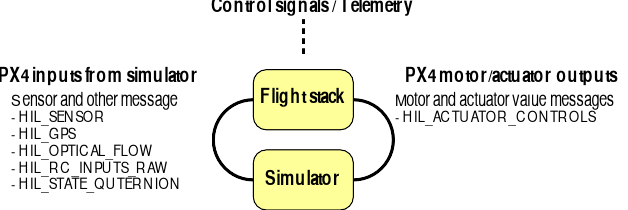
\includegraphics[width=0.70\textwidth]{../media/px4.png}
    \caption{PX4 interface graphic (source asset: \texttt{../media/px4.svg}, rasterized to PNG for pdflatex compatibility).}
    \label{fig:px4_interface}
\end{figure}

\begin{itemize}
    \item \texttt{HIL\_SENSOR} at simulation update rate,
    \item \texttt{HIL\_GPS} on GPS update events,
    \item \texttt{HIL\_STATE\_QUATERNION} when requested by \texttt{MAV\_CMD\_SET\_MESSAGE\_INTERVAL},
    \item \texttt{SYSTEM\_TIME} and periodic heartbeat.
\end{itemize}

\subsubsection*{Lockstep Message Sequence}
{\footnotesize
\begin{verbatim}
Init defaults in main.py:
  sim_time_us = 0
  now_ms = sim_time_us // 1000
  RATE_HZ = 250, DT_US = 4000
  slow_down_counter = 0, CHECK_FACTOR = 2
  hil_state_interval_us = -1      (HIL_STATE_QUAT disabled)
  gps_start_time_us = 1_000_000us (1 s delay)

PX4                   Bridge(main.py)                World/Sensors
 |                          |                               |
 |-- HEARTBEAT -----------> |                               |
 |-- HIL_ACTUATOR_CTRL ---> |                               |
 |-- COMMAND_LONG (opt) --> |                               |
 |                          |-- parse RX MAVLink ---------->|
 |                          |<-- controls + arming ---------|
 |                          |                               |
 |                          | local standalone/master mode: |
 |                          |   sim_time_us += DT_US        |
 |                          |   ioOnlyRun = (slow_down_counter % 2 != 0)
 |                          |   if ioOnlyRun: I/O-only cycle
 |                          |      (skip full dynamics step)
 |                          |   else world.update(...) ----->|
 |                          |        <- y, ydot, sensors ----|
 |                          |   slow_down_counter += 1        |
 |                          |                               |
 |<-- HIL_SENSOR ---------- | from SensorSuite publish path  |
 |<-- HIL_STATE_QUAT* ----- | from state y                  |
 |<-- HIL_GPS** ----------- | from SensorSuite GPS output    |
 |<-- SYSTEM_TIME (1Hz) ----|                               |
 |<-- HEARTBEAT (1Hz) ------|                               |
 |                          |-- sleep(1/RATE_HZ), next loop |

* HIL_STATE_QUAT default: OFF (hil_state_interval_us = -1)
  Enabled by MAV_CMD_SET_MESSAGE_INTERVAL for msg id 115.

** HIL_GPS default send condition:
   sim_time_us >= gps_start_time_us AND gps_updated == true.

Note: sim_time_us is incremented before ioOnlyRun is evaluated, so it advances
      even during I/O-only cycles.
\end{verbatim}
}

Simulation-step timing rule in standalone/master mode:
\begin{equation}
t_{k+1} = t_k + \Delta t, \quad \Delta t = \frac{1}{\text{RATE\_HZ}}.
\end{equation}

\subsection{Ground Truth WebSocket}
\texttt{src/networking/websocket_publisher.py} streams JSON ground-truth state for external visualizers and analysis tools.

\section{Python Installation and Interaction}
\subsection{Install}
This repository is installable as a Python package (see \texttt{pyproject.toml}).
\begin{verbatim}
python -m pip install -e .
\end{verbatim}
The console entry point is:
\begin{verbatim}
px4-python-sitl
\end{verbatim}

\subsection{Run from CLI}
Typical usage is to start the bridge and connect it to PX4 SITL over MAVLink.
\begin{verbatim}
px4-python-sitl --help
python src/main.py --help
\end{verbatim}
\subsection{Interact from Python}
You can import simulation modules and run/update components programmatically.
\begin{verbatim}
from vehicle.world import World

world = World(vehicle_model="iris")

# set controls/wind, advance lockstep, read state/sensors
world.set_controls([0.0, 0.0, 0.0, 0.0])
world.set_wind([0, 0, 0, 0, 0, 0])
out = world.update(t_us=4000, paused=False)
print(out["y"])         # state
print(out["sensors"])   # synthesized sensors
\end{verbatim}

\subsection{External Program Interfaces}
\begin{itemize}
    \item MAVLink HIL I/O via \texttt{src/main.py}.
    \item Ground-truth WebSocket via \texttt{src/networking/websocket_publisher.py}.
\end{itemize}

\section{Build and Use}
The document can be built with:
\begin{verbatim}
make -C docs
\end{verbatim}
or directly:
\begin{verbatim}
pdflatex -output-directory docs docs/architecture.tex
\end{verbatim}

\end{document}
